%!TEX root = ../report.tex

\chapter{Active Learning}

Active learning is a special case of semi-supervised machine learning in which a learning algorithm is able to interactively query the user to obtain the desired outputs at new data points. \cite{active_learning}

Supervised learning performs well when the model is trained with a large number of labeled instances.  But the labeled instances are very difficult, time-consuming, or expensive to obtain.  Active learning helps in overcoming the situations where there is plenty of unlabeled data is available which are difficult to label or the cost of labeling them is high.  The main aim of the active learning is to improve the accuracy by labeling less number of instances. The instances that need to be labeled is determined by the active learning query strategies.\cite{Settles2010}

\begin{figure}[h!]
	\centering
	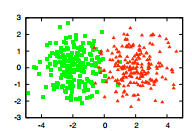
\includegraphics[scale=1]{images/sample_data}
	\caption{Sample data points  in a 2D feature space  \cite{Settles2010}.}
	\label{sample_data}
\end{figure}

Let us consider the Fig \ref{sample_data}. It consists of 400 data points in a 2D feature space generated using two Gaussian centered  (-2,0) and (2,0) with standard deviation $\sigma$ = 1.  These data points belong to two classes. (each class has 200 data points).

\begin{figure}[h!]
	\centering
	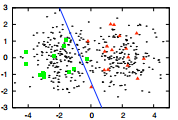
\includegraphics[scale=1]{images/random_sampling}
	\caption{Decision boundary obtained by random sampling \cite{Settles2010}.}
	\label{random_sampling}
\end{figure}

Fig \ref{random_sampling} shows the decision boundary obtained using a supervised learning approach after selecting 30 data points randomly for labeling. The line denotes the linear decision boundary of a logistic regression model is sub-optimal. This model achieves 70 \% accuracy on the remaining unlabeled points because of the poor selection of data points for labeling.

\begin{figure}[h!]
	\centering
	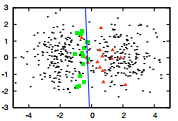
\includegraphics[scale=1]{images/active_sampling}
	\caption{Decision boundary obtained by sampling using active learnig strategies \cite{Settles2010}.}
	\label{active_sampling}
\end{figure}


Fig \ref{active_sampling} shows the decision boundary obtained using active learning approach. The active learning approach selects 30 points close to the decision boundary for labeling. By using the label for these data points, the classifier achieves 90 \% accuracy which is significantly better than the approach by random sampling of data points. \cite{Settles2010}

\section{Active Learning Scenarios:}


There are three main problem scenario that can occur when the learner queries the user. They are 
\begin{itemize}
\item membership query synthesis
\item stream-based selective sampling
\item pool-based sampling
\end{itemize}

\subsection{Membership query synthesis:}
	In this scenario, the learner is allowed to choose any unlabeled data points which can include the a new query that the learner generates instead of the data points sampled from the underlying distribution. \\
\begin{figure}[h!]
	\centering
	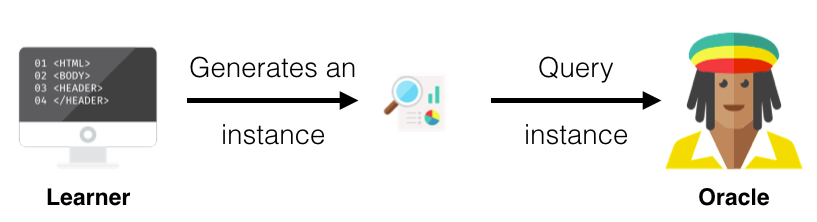
\includegraphics[scale=0.4]{images/membership}
	\caption{Membership query synthesis \cite{active_learning_datacamp}.}
	\label{membership}
\end{figure}\\
Fig \ref{membership} shows the workflow of membership query synthesis.The shortcoming of this setting is that the query generated by the learner can sometimes be unrecognized for the human to label. When applying this setting to the task of handwritten classification, the learner generates hybrid characters that no natural semantic meaning. \cite{Settles2010}
\subsection{Stream-based selective sampling:}
    In this setting, the instances are drawn from the data source in a sequence and the learner decide whether to query this particular instance or not. \\
\begin{figure}[h!]
	\centering
	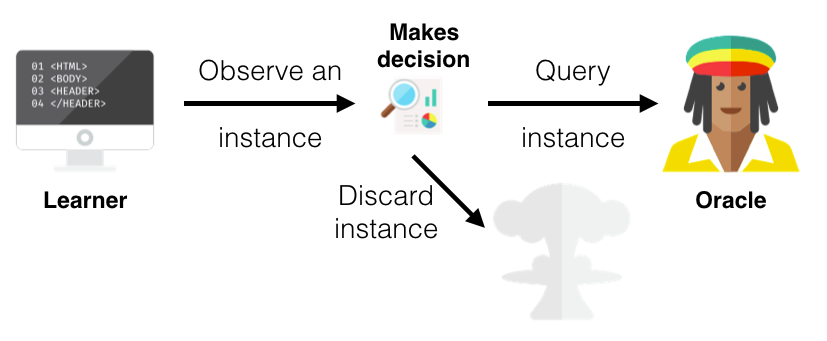
\includegraphics[scale=0.4]{images/stream_based}
	\caption{Stream-based selective sampling \cite{active_learning_datacamp}.}
	\label{stream_based}
\end{figure}\\
Fig \ref{stream_based} shows the workflow of membership query synthesis.The decision on querying the instance is decided by various query strategies that will be discussed in the upcoming section. \cite{Settles2010}
    
\subsection{Pool-Based Sampling:}
	The pool-based labeling setting consists of two pools of data which include a large set of unlabeled data and a small set of labeled ones. The instances are queried based on the usefulness to evaluate the other instances in the unlabeled pool.\\
\begin{figure}[h!]
	\centering
	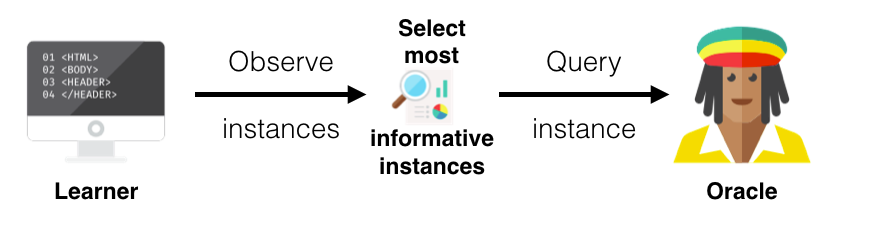
\includegraphics[scale=0.4]{images/pool_based}
	\caption{Pool-based selective sampling \cite{active_learning_datacamp}.}
	\label{pool_based}
\end{figure}\\
Fig \ref{pool_based} shows the workflow of membership query synthesis.It has been used in a wide range of real-world problems such as text classification, information extraction, image classification and retrieval, video classification and retrieval and speech recognition. \cite{Settles2010}

\section{Query strategy frameworks:}
	
Passive learning approach has a large amount of labeled data which are sampled from an underlying distribution is used to train a model. Then the trained model is used for prediction. But in active learning, the learner query the most informative instance or the best instance which is the main difference between active and passive learning. There are various strategies to select the most informative query which are discussed below. \cite{Settles2010}

\subsection{Uncertainty Sampling:}
   Uncertainty Sampling is the most commonly used query strategy framework. Here, the learner queries the most uncertain instance. There are three subdivisions of uncertainty sampling which includes 
\subsubsection{Least confident uncertainty sampling:} 
	In the least confident uncertainty sampling, the most uncertain instance is selected. The uncertainty measure of the particular sample is the uncertainty of the class label with the highest posterior probability. The sample whose uncertainty is more is queried.  \\
\begin{table}[h]
\centering
\begin{tabular}{llll}
Datapoints & Class A & Class B & Class C \\
D1         & 0.1     & 0.8     & 0.2     \\
D2         & 0.35    & 0.15    & 0.50   
\end{tabular}
\end{table} \\
	In the above table, the uncertainty of data point D1  is the uncertainty  of the class label with the highest posterior probability which is 0.2  and similarly for D1, it will be 0.5. It is clear that the data point D2 is more uncertain which will be queried. \cite{Settles2010}\cite{modal}
\subsubsection{Margin uncertainty sampling:}
	Least confident strategy only considers information about the most probable label thereby it ignores the information about the other label information. In margin uncertainty sampling, it considers the first two most probable labels and their difference is used to determine the margin. The data points with less margin are considered here and it is queried. \\
\begin{table}[h]
\centering
\begin{tabular}{llll}
Datapoints & Class A & Class B & Class C \\
D1         & 0.1     & 0.7     & 0.3     \\
D2         & 0.35    & 0.10    & 0.55   
\end{tabular}
\end{table} \\
In the above example, the data point D1 has a margin size of 0.4 (0.7 – 0.3) and for data point D2, the margin size will be 0.2(0.55 – 0.35) . The data point D2 has the least margin between the most likely predicted labels. Hence data point D2 will be queried. \cite{Settles2010}\cite{modal}
\subsubsection{Entropy uncertainty sampling:}   
	The most general and popular uncertainty sampling measure is entropy sampling. The volume of information needed to encode a distribution is represented as an information theoretic measure which is termed as entropy. Both the least confident and margin based strategies select the instance that has a posterior class probability close to 0.5. But the advantage of entropy-based selection generalizes easily to probabilistic multi-label classifiers. \cite{Settles2010}\cite{modal}
	
\subsection{Query-By-Committee:}
\subsection{Expected Model Change:}
\subsection{Expected Error Reduction:}
\subsection{Variance Reduction:}
\subsection{Density-Weighted Methods:}
\subsection{Uncertainty Sampling:}